\documentclass{ctexart}
\usepackage[T1]{fontenc}
\usepackage[a4paper,top=1.5cm,bottom=1.5cm,left=2cm,right=2cm,marginparwidth=1.75cm]{geometry}
\usepackage{mathtools}
\usepackage{tikz}
\usepackage{booktabs}
\usepackage{caption}
\usepackage{outlines}
\usepackage{graphicx}
\usepackage{float}
\usepackage{amsthm}
\usepackage{tabularray}
\usepackage{underscore}
\usepackage{minted}
\usepackage[colorlinks=false, allcolors=blue]{hyperref}
\usepackage{cleveref}
\renewcommand{\tableautorefname}{表}
\UseTblrLibrary{booktabs}
\DeclarePairedDelimiter{\set}{\{}{\}}
\DeclarePairedDelimiter{\paren}{(}{)}
\graphicspath{ {./images/} }
\crefname{equation}{方程}{方程}
\crefname{algorithm}{算法}{算法}
\crefname{lemma}{引理}{引理}
\crefname{table}{表}{表}
\crefname{figure}{图}{图}
\crefname{example}{例}{例}

\newcounter{fullrefcounter}
\newcommand*{\fullref}[1]{%
\addtocounter{fullrefcounter}{1}%
\label{--ref-\thefullrefcounter}%
\ifthenelse{\equal{\getpagerefnumber{--ref-\thefullrefcounter}}{\getpagerefnumber{#1}}}
  {
    \hyperref[{#1}]{\Cref*{#1} \nameref*{#1}}
  }
  {% false case
    \hyperref[{#1}]{第 \pageref*{#1} 页 \Cref*{#1} \nameref*{#1}}
  }
}
\newcommand{\todo}[1]{({\color{red} TODO: #1 })}

\title{计算机网络系统设计}
\author{卢雨轩 19071125 \\ 孙天天 19071110 \\ 刘~~~阳 19071127}
% \date{\today}
\ctexset{
    section = {
        titleformat = \raggedright,
        name = {,},
        number = \chinese{section}、
    },
    paragraph = {
        runin = false
    },
    today = small,
    figurename = 图,
    contentsname = 目录,
    tablename = 表,
}

\begin{document} 

\maketitle

\section{总体设计}
采用Rust编写ping程序。在解析用户传入的命令行参数后,使用netlink系统调用获取系统路由表(也可以选择绕过路由表),使用pnet库提供的raw网络接口构造ICMP和IP数据包并发送。发送一个数据包的典型流程见 \cref{fig:ping-flow}。

\begin{figure}[htp]
    \centering
    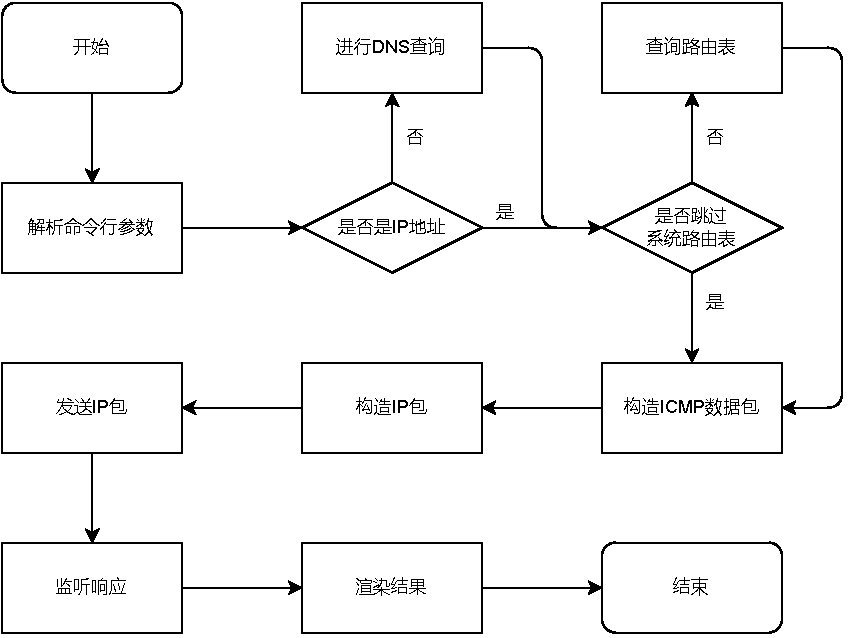
\includegraphics[width=.8\linewidth]{design.drawio.pdf}
    \caption{发送一个数据包的典型流程}
    \label{fig:ping-flow}
\end{figure}

预计实现以下功能:
% 基础ping、traceroute、画图(统计图+拓扑图)
\iffalse

Usage
  ping [options] <destination>

Options:
  <destination>      dns name or ip address
  -a                 use audible ping
  -A                 use adaptive ping
  -B                 sticky source address
  -c <count>         stop after <count> replies
  -D                 print timestamps
  -f                 flood ping
  -h                 print help and exit
  -I <interface>     either interface name or address
  -i <interval>      seconds between sending each packet
  -L                 suppress loopback of multicast packets
  -l <preload>       send <preload> number of packages while waiting replies
  -m <mark>          tag the packets going out
  -M <pmtud opt>     define mtu discovery, can be one of <do|dont|want>
  -n                 no dns name resolution
  -O                 report outstanding replies
  -p <pattern>       contents of padding byte
  -q                 quiet output
  -Q <tclass>        use quality of service <tclass> bits
  -s <size>          use <size> as number of data bytes to be sent
  -S <size>          use <size> as SO_SNDBUF socket option value
  -t <ttl>           define time to live
  -U                 print user-to-user latency
  -v                 verbose output
  -V                 print version and exit
  -w <deadline>      reply wait <deadline> in seconds
  -W <timeout>       time to wait for response

IPv4 options:
  -4                 use IPv4
  -b                 allow pinging broadcast
  -R                 record route
  -T <timestamp>     define timestamp, can be one of <tsonly|tsandaddr|tsprespec>

IPv6 options:
  -6                 use IPv6
  -F <flowlabel>     define flow label, default is random
  -N <nodeinfo opt>  use icmp6 node info query, try <help> as argument

\fi
\begin{outline}
    \1 基础ping的网络测试功能,包含Linux的ping软件中较为具有代表性的功能。
        \2 如:广播地址、设置TTL、安静模式、包数量、包大小等
    \1 traceroute:通过不断增加发的包的TTL,根据返回的TimeExceeded包的源地址来跟踪从当前机器到目标机器的路由链路。通过geoip服务获取ip地址的地理位置信息并展示。
    \1 CLI图像绘制功能:绘制拓扑意义上的网络连接图和统计意义上的延迟折线图,来更形象地展示网络测试结果。
\end{outline}

\section{ICMP部分}
本功能块负责构造ICMP Echo Reqest包。相关代码如下:
\begin{minted}[breaklines]{rust}
let mut vec: Vec<u8> = vec![0; 16]; // 包长度
// Use echo_request so we can set the identifier and sequence number
let mut echo_packet = echo_request::MutableEchoRequestPacket::new(&mut vec[..]).unwrap();
echo_packet.set_sequence_number(20); // SEQ字段
echo_packet.set_identifier(2);       // Ident字段
echo_packet.set_icmp_type(IcmpTypes::EchoRequest);

let csum = util::checksum(echo_packet.packet(), 1);
echo_packet.set_checksum(csum);
\end{minted}

\section{TCP部分}
本模块负责构造IP数据包。相关代码如下:
\begin{minted}{rust}

let mut ip_vec: Vec<u8> = vec![0; Ipv4Packet::minimum_packet_size() + 16];
let mut ip_packet = MutableIpv4Packet::new(&mut ip_vec[..]).unwrap();

let total_len = (20 + 16) as u16;

ip_packet.set_version(4);
ip_packet.set_header_length(5);
ip_packet.set_total_length(total_len);                      // 总长度
ip_packet.set_ttl(128);                                     // TTL
ip_packet.set_next_level_protocol(IpNextHeaderProtocols::Icmp); // ICMP协议
ip_packet.set_source(Ipv4Addr::new(172, 31, 135, 147));     // 源地址
ip_packet.set_destination(Ipv4Addr::new(172, 31, 143, 255));// 目标地址

let checksum = ipv4::checksum(&ip_packet.to_immutable());
ip_packet.set_checksum(checksum);                           // 计算校验码
ip_packet.set_payload(echo_packet.packet());
\end{minted}

\section{CLI图像绘制部分}
本课设支持的CLI图像绘制模块旨在直观地展示网络环境状况。具体地说,系统支持绘制网络连接的拓扑结构图和延迟测试折线统计图。

\subsection{网络连接拓扑结构图}
我们利用来自于多次traceroute和ping得到的数据绘制网络中各设备的拓扑关系图。用户可以开关是否要将接下来的测试结果放入拓扑结构图的绘制中。

使用类似git提交结点可视化的方式,效果大致如下所示。

\begin{minted}{text}
* 10.0.0.2 (内网)
|
* 10.0.0.1 (内网)
|\
* | 114.5.14.19 (北京市 北京 联通)
| * 19.8.1.0 (北京市 北京 联通)
|\ \ 
* | | 218.197.48.78 (湖北省 十堰市 教育网)
  * | 11.45.1.4 (美国 俄亥俄)
    * 191.9.8.10 (巴西)
\end{minted}


\subsection{延迟折线统计图}
我们计划用折线统计图的方式实时显示最近几次ping的延迟数据,这样可以直观地观察延迟变化。

\begin{figure}[h]
  \centering
  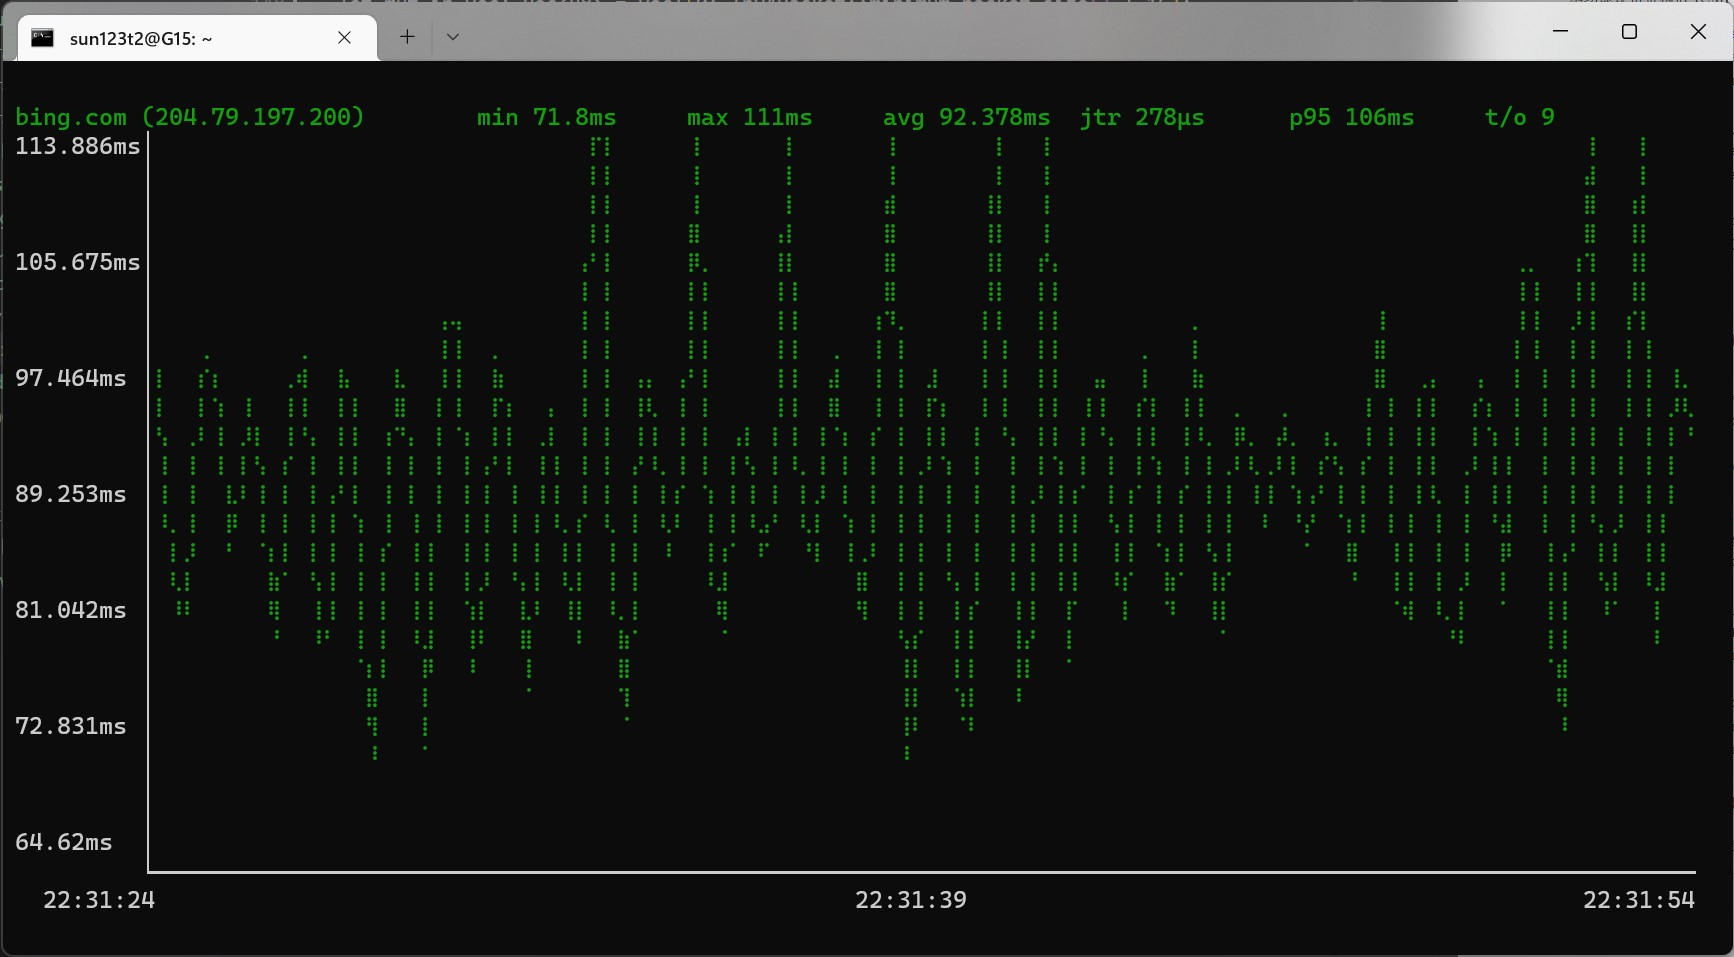
\includegraphics[width=\linewidth]{gping.jpg}
  \caption{延迟折线统计图设想图示}
  \label{image:gping}
\end{figure}

效果大致如图\ref{image:gping}所示,当统计图未填满终端时从左边向右生长,填满时则整体向左平移滚动显示。

\end{document}
